\chapter{Laboratorium 3}
\label{cha:Lab003}
\makeatletter


% *********************************************************************
% w poniższej metryczce należy uzupełnić informacje o:
% - temacie ćwiczenia
% - numer ćwiczenia
% - numer grupy laboratoryjnej
% - numer zespołu
% - datę wykonania ćwiczenia oraz oddania ćwiczenia.
% *********************************************************************

\begin{table}[H]
    \centering
    \renewcommand{\tabularxcolumn}[1]{m{#1}}  % Dostosowanie kolumny do zawartości
    \newcolumntype{C}{>{\centering\arraybackslash}X}
    \begin{tabularx}{\linewidth}{|C|C|}
        \hline
        \multicolumn{2}{|c|}{\makecell{\textbf{\Large{Biometryczne Systemy Zabezpieczeń}} \\ \textbf{Ćwiczenia Laboratoryjne}}} \\ \hline
        \multicolumn{1}{|l|}{Temat}                    &              OPERACJE MORFOLOGICZNE NA OBRAZACH            \\ \hline
        \multicolumn{1}{|l|}{Ćwiczenie nr:}                    &      03                   \\ \hline
        \multicolumn{1}{|l|}{Autorzy:}                         &   \@author                              \\ \hline
        \multicolumn{1}{|l|}{Grupa laboratoryjna}                       &       02               \\ \hline
        \multicolumn{1}{|l|}{Zespół nr. }                       &    XX                  \\ \hline
        \multicolumn{1}{|l|}{Data wykonana ćwiczenia}         &  26.04.2025     \\ \hline
        \multicolumn{1}{|l|}{Data oddania ćwiczenia  }         &   13.05.2025     \\ \hline
    \end{tabularx}
\end{table}


\section{Cel ćwiczenia}

Operacje morfologiczne są kluczowym narzędziem w przetwarzaniu obrazów, szczególnie w analizie
kształtów i struktury obiektów. Dzięki wykorzystaniu odpowiednich elementów strukturalnych można
dostosować te operacje do różnych zadań, takich jak segmentacja, poprawa jakości obrazu czy analiza
konturów. Celem laboratorium jest zapoznanie się z operacjami morfologicznymi na obrazach.

\section{Wstęp teoretyczny}

Operacje morfologiczne to techniki przetwarzania obrazów stosowane głównie do analizy kształtu i struktury obiektów w obrazach binarnych oraz, w pewnym stopniu, w obrazach w skali szarości. Ich główną cechą jest wykorzystanie elementów strukturalnych do modyfikowania obrazu.

\textbf{Szkieletyzacja} to proces odnoszący się do ścieniania linii konturowych obiektu, który znalazł zastosowanie w wielu dziedzinach, takich jak:
\begin{itemize}
	\item medycyna (analiza białych ciałek krwi, chromosomów, naczyń wieńcowych),
	\item kryminalistyka (rozpoznawanie odcisków palców),
	\item przemysł elektroniczny (analiza obwodów drukowanych),
	\item wektoryzacja obrazów rastrowych.
\end{itemize}

W niniejszym opracowaniu przedstawiono sposób działania wybranych algorytmów szkieletyzujących: Arcelli-Levialdi-Pavlidis, Chin-Van-Stover-Iverson oraz Rosenfeld-Peleg. Zaprojektowano także aplikację umożliwiającą użytkownikowi wprowadzanie własnych szablonów szkieletyzujących oraz obserwowanie otrzymanych wyników.

\subsection{Szkieletyzacja obrazów binarnych}

Spośród klasycznych metod ścieniania (\textit{skeletoning} lub \textit{thinning algorithms}), wyróżnić można trzy główne podejścia:
\begin{itemize}
	\item \textbf{Wypełnianie działów wodnych} (dla obrazów w skali szarości),
	\item \textbf{Hit or Miss Transform} (dla obrazów binarnych i szarych),
	\item \textbf{Medial Axis Transform} (posiadająca przekształcenie odwrotne).
\end{itemize}

Podstawą tych metod są dwa główne przekształcenia morfologiczne: erozja i dylatacja. Formalnie, dla obrazów binarnych:

\begin{equation}
	A \oplus B = \bigcup_{b \in B} \left( \bigcup_{a \in A} (a + b) \right)
\end{equation}

\begin{equation}
	A \ominus B = \bigcap_{b \in B} \left( \bigcup_{a \in A} (a + b) \right)
\end{equation}

gdzie $A$ to obraz, $B$ to maska (element strukturalny), $\oplus$ oznacza dylatację, a $\ominus$ erozję. Znak $\bigcup$ oznacza sumę zbiorów, a $\bigcap$ ich część wspólną.

Hit or Miss Transform można opisać następująco:
\begin{itemize}
	\item przykładamy element strukturalny $b$ do każdego punktu obrazu,
	\item jeśli $b$ pokrywa się z sąsiedztwem - zmieniamy wartość piksela (zwykle na 0),
	\item w przeciwnym wypadku piksel pozostaje niezmieniony.
\end{itemize}

Algorytmy takie jak Arcelli-Levialdi stosują szablony operujące na oknie bieżącego piksela oraz jego ośmiu sąsiadów. Możliwa jest także modyfikacja szablonów (np. użycie bitów typu "don't care") w celu uzyskania lepszego efektu szkieletyzacji gałęzi pionowych.

\subsection{Algorytm Chin-Van-Stover-Iverson}

Algorytm CVSI porównuje sąsiedztwo piksela z zestawem szablonów (1--8). Jeśli spełniony jest warunek zgodności z szablonem, następuje dodatkowe porównanie z szablonami 9 i 10. 

\begin{itemize}
	\item Jeśli otoczenie nie różni się od żadnego z szablonów — piksel pozostaje (jest częścią szkieletu).
	\item Jeśli różni się — piksel zostaje usunięty.
\end{itemize}

Aplikacja umożliwia ręczną edycję szablonów przez użytkownika (zmiana wartości 0, 1, x za pomocą kliknięć).

\subsection{Szkieletyzacja obrazów tonowanych}

Naturalnym rozwinięciem szkieletyzacji obrazów binarnych jest szkieletyzacja obrazów w skali szarości. Przykładowe podejścia:

\begin{itemize}
	\item erozja (Rosenfeld-Peleg),
	\item przekształcenie typu top-hat.
\end{itemize}

Ogólna translacja sygnału $f(x)$:

\begin{equation}
	f(x) = f(x - z)
\end{equation}

\begin{equation}
	(f \oplus y)(x) = f(x) + y
\end{equation}

Obie translacje można łączyć:

\begin{equation}
	(f_z \oplus y)(x) = f(x - z) + y
\end{equation}

Jeśli przyjmiemy, że $f(x) = -\infty$ poza obrazem, to dziedzinę obrazu określimy jako:

\begin{equation}
	D[f] = \{x : f(x) > -\infty\}
\end{equation}

Jeżeli $g(x) \leq f(x)$ dla każdego $x$, to:

\begin{equation}
	D[g] \subseteq D[f]
\end{equation}

Erozję definiujemy jako:

\begin{equation}
	(f \wedge g)(x) = 
	\begin{cases}
		\min\{f(x), g(x)\}, & x \in D[f] \cap D[g] \\
		-\infty, & \text{inaczej}
	\end{cases}
\end{equation}

Przy zastosowaniu płaskiego elementu strukturyzującego ($g_z(x) = 0$), erozję można zapisać jako:

\begin{equation}
	(f \ominus g)(x) = \min\{f(x) - g_z(x)\}
\end{equation}

co odpowiada filtracji typu \textit{moving minimum}.

Do obserwacji zachowania algorytmu Rosenfeld-Peleg zaprojektowano obraz syntetyczny zawierający cylindryczną falę sinusoidalną.

\section{Zadania do wykonania samodzielnego}

\subsection{Zadanie 1}

\subsubsection{Treść}

\begin{enumerate}
	\item Załaduj obraz testowy oraz przygotuj obraz do realizacji dalszych ćwiczeń o rozmiarach:
	\item Wykonaj program realizujący algorytm ścieniania, którego zestaw kerneli zamieszczono poniżej:
	\item Do zaprogramowania kolejnych szablonów i masek wykorzystaj poniższy fragment kodu źródłowego (funkcja intbin8 formuje 8-bitową reprezentację liczby dziesiętnej przekazywanej parametrem i):
	\item Sprawdź poprawność działania algorytmu na innym obrazie testowym, dla zmodyfikowanych
	parametrów filtracji morfologicznej jak poniżej:
	\item Wyświetl wyniki otrzymanych filtracji wraz z podpisem w oknie wykorzystując funkcję subplot.
	\item Wyjaśnij zjawisko zmieniającej się szybkości wykonywania algorytmu w zależności od fazy jego wykonywania.
	\item Wykonaj wersję algorytmu realizującego szkieletyzację wg Chin-Wan-Stover-Iverson, przyjmując zestaw kerneli jak poniżej
	\item Przeprowadź dyskusję otrzymanych wyników jak dla pkt 5-6.
\end{enumerate}

\subsubsection{Przykładowy program}

\lstinputlisting[style= matlabStyle, caption= Wczytanie obrazu i stworzenie konwersji, label=Lab003_l1]{src/Lab003/zadanie1.m}

\subsubsection{Obrazy}

\begin{figure}[H]
	\centering
	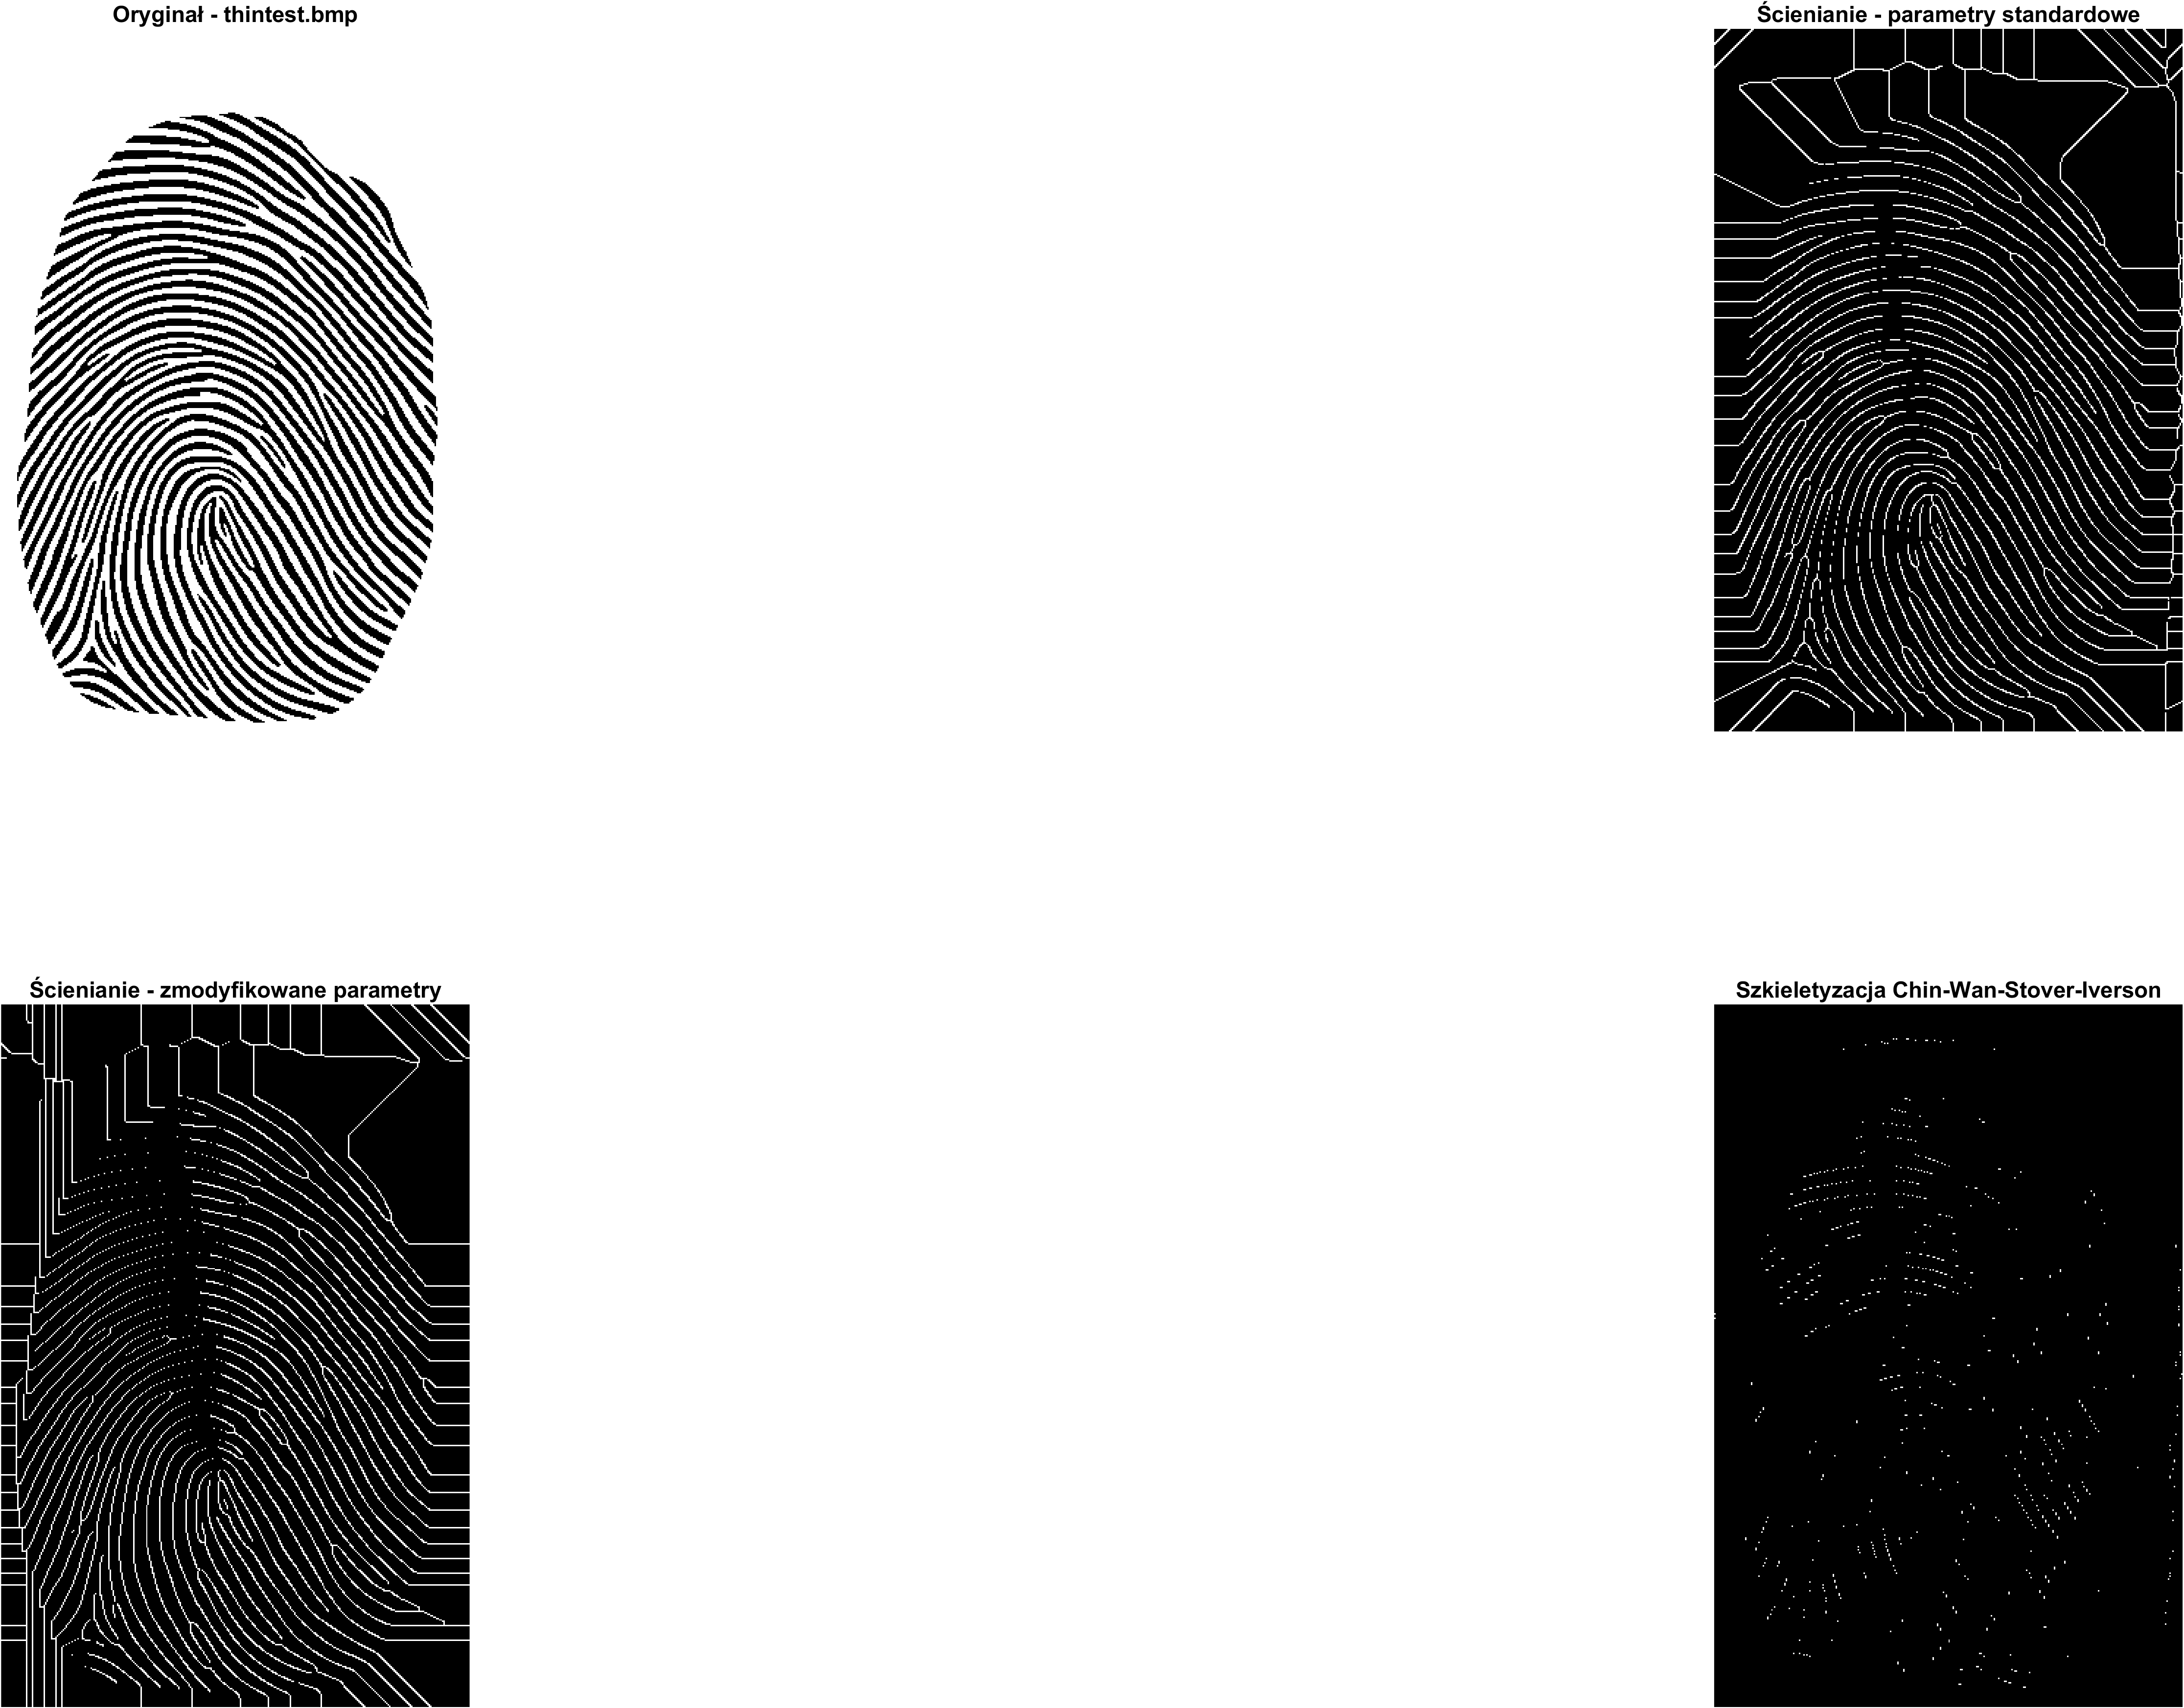
\includegraphics[width=0.8\textwidth]{src/Lab003/results.png}
	\caption{Porównanie wyników: Oryginał, Ścienianie standardowe, Ścienianie zmodyfikowane, Szkieletyzacja CWSI.}
\end{figure}

\section{Wnioski}

W przeprowadzonym ćwiczeniu dokonano analizy działania dwóch metod ścieniania obrazów binarnych:

\begin{itemize}
	\item Metody klasycznej ścieniania z wykorzystaniem standardowych oraz zmodyfikowanych masek.
	\item Metody szkieletyzacji Chin-Wan-Stover-Iverson.
\end{itemize}

Na podstawie uzyskanych wyników można wyciągnąć następujące wnioski:

\begin{enumerate}
	\item \textbf{Ścienianie z maskami standardowymi} pozwala na sukcesywne usuwanie zbędnych pikseli z obrazu, prowadząc do uzyskania cieńszych struktur. Proces ten jest stosunkowo stabilny, zachowując kształt linii papilarnych.
	
	\item \textbf{Zmodyfikowane parametry ścieniania} powodują bardziej agresywne usuwanie pikseli. Widoczne jest zwiększone uproszczenie obrazu, jednak miejscami może to prowadzić do zniekształcenia struktury oryginalnych linii.
	
	\item \textbf{Szkieletyzacja metodą Chin-Wan-Stover-Iverson} skutkuje szybkim i skutecznym redukowaniem obrazu do jego podstawowych konturów. Uzyskany szkielet jest bardzo cienki, jednak często prowadzi do fragmentacji obrazu, zwłaszcza w miejscach o większej gęstości pikseli.
	
	\item \textbf{Szybkość działania algorytmu} jest największa na początku, gdy usuwane są większe grupy pikseli. W późniejszych iteracjach proces znacznie zwalnia, ponieważ zmiany obejmują pojedyncze piksele.
	
	\item Obie metody pozwalają na skuteczne ścienianie obrazów binarnych, jednak wybór odpowiedniej metody oraz parametrów powinien być dostosowany do specyfiki przetwarzanego obrazu oraz wymagań aplikacji końcowej (np. analizy odcisków palców, rozpoznawania wzorców itp.).
\end{enumerate}

Dzięki zastosowaniu różnych wariantów masek oraz metod możliwe jest dostosowanie procesu ścieniania do indywidualnych potrzeb, co stanowi istotny aspekt w cyfrowym przetwarzaniu obrazów.